% tikz_diagram.tex
% Flowchart and diagram examples using TikZ
% Demonstrates nodes, arrows, positioning, and diagram creation

\documentclass[12pt,a4paper]{article}

\usepackage{tikz}
\usepackage[margin=1in]{geometry}

% TikZ libraries for flowcharts and diagrams
\usetikzlibrary{
    shapes.geometric,
    shapes.multipart,
    arrows.meta,
    positioning,
    calc,
    fit,
    backgrounds
}

\title{TikZ Flowcharts and Diagrams}
\author{LaTeX Student}
\date{\today}

\begin{document}

\maketitle

\section{Simple Flowchart}

\begin{center}
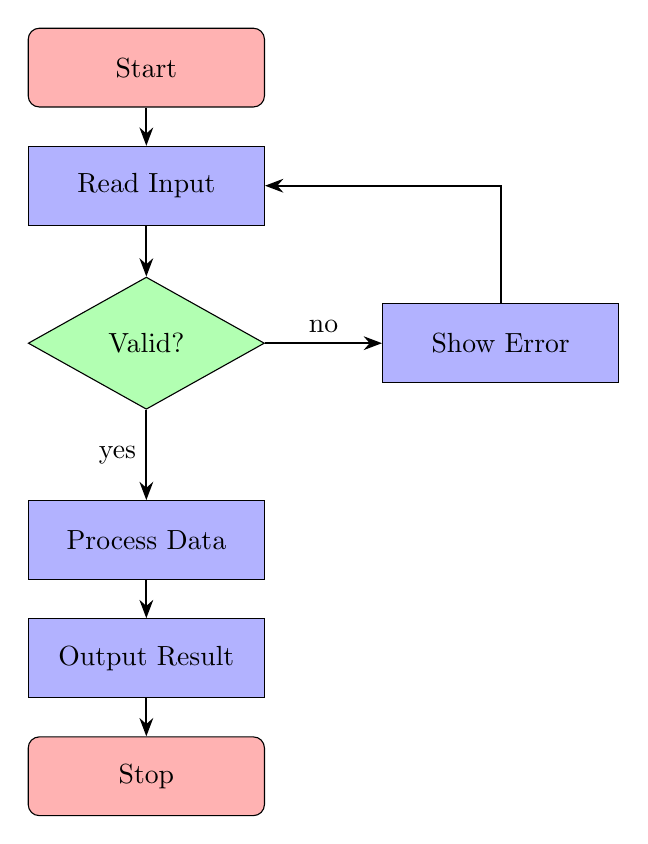
\begin{tikzpicture}[
    node distance=1.5cm,
    startstop/.style={rectangle, rounded corners, minimum width=3cm, minimum height=1cm,
                      text centered, draw=black, fill=red!30},
    process/.style={rectangle, minimum width=3cm, minimum height=1cm,
                    text centered, draw=black, fill=blue!30},
    decision/.style={diamond, minimum width=3cm, minimum height=1cm,
                     text centered, draw=black, fill=green!30},
    arrow/.style={thick,->,>=Stealth}
]

    % Nodes
    \node (start) [startstop] {Start};
    \node (input) [process, below of=start] {Read Input};
    \node (decide) [decision, below of=input, yshift=-0.5cm] {Valid?};
    \node (process1) [process, below of=decide, yshift=-1cm] {Process Data};
    \node (error) [process, right of=decide, xshift=3cm] {Show Error};
    \node (output) [process, below of=process1] {Output Result};
    \node (stop) [startstop, below of=output] {Stop};

    % Arrows
    \draw [arrow] (start) -- (input);
    \draw [arrow] (input) -- (decide);
    \draw [arrow] (decide) -- node[anchor=east] {yes} (process1);
    \draw [arrow] (decide) -- node[anchor=south] {no} (error);
    \draw [arrow] (error) |- (input);
    \draw [arrow] (process1) -- (output);
    \draw [arrow] (output) -- (stop);

\end{tikzpicture}
\end{center}

\section{Algorithm Flowchart}

\begin{center}
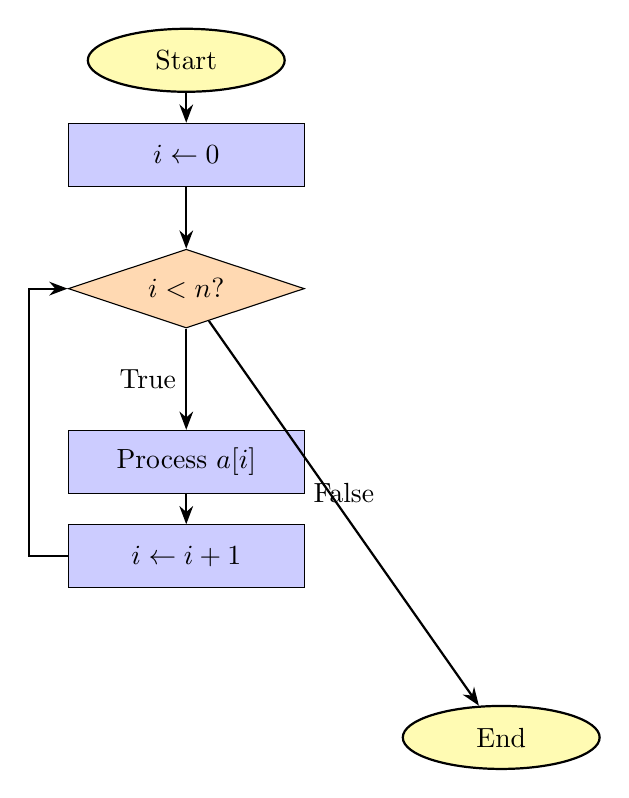
\begin{tikzpicture}[
    node distance=1.2cm,
    start/.style={ellipse, minimum width=2.5cm, minimum height=0.8cm,
                  text centered, draw=black, fill=yellow!30, thick},
    block/.style={rectangle, minimum width=3cm, minimum height=0.8cm,
                  text centered, draw=black, fill=blue!20},
    condition/.style={diamond, aspect=2.5, minimum width=3cm, minimum height=1cm,
                      text centered, draw=black, fill=orange!30},
    arrow/.style={->,>=Stealth,thick}
]

    \node (start) [start] {Start};
    \node (init) [block, below of=start] {$i \leftarrow 0$};
    \node (check) [condition, below of=init, yshift=-0.5cm] {$i < n$?};
    \node (process) [block, below of=check, yshift=-1cm] {Process $a[i]$};
    \node (increment) [block, below of=process] {$i \leftarrow i + 1$};
    \node (end) [start, below of=check, yshift=-4.5cm, xshift=4cm] {End};

    \draw [arrow] (start) -- (init);
    \draw [arrow] (init) -- (check);
    \draw [arrow] (check) -- node[anchor=east] {True} (process);
    \draw [arrow] (process) -- (increment);
    \draw [arrow] (increment) -| ++(-2,0) |- (check);
    \draw [arrow] (check) -- node[anchor=south] {False} (end);

\end{tikzpicture}
\end{center}

\section{System Architecture Diagram}

\begin{center}
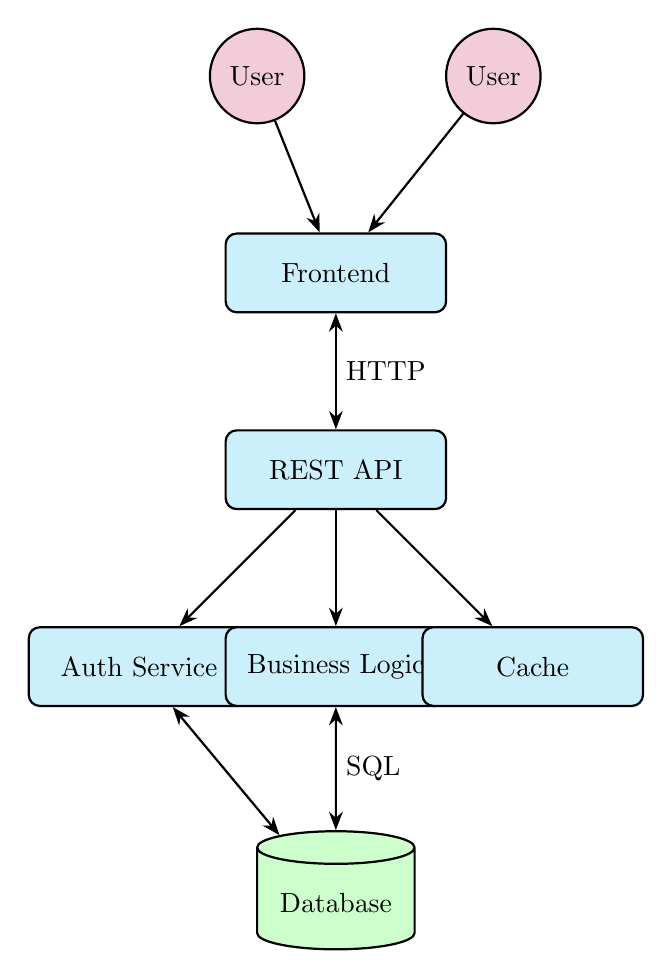
\begin{tikzpicture}[
    node distance=2cm,
    component/.style={rectangle, rounded corners, minimum width=2.8cm, minimum height=1cm,
                      text centered, draw=black, thick, fill=cyan!20},
    database/.style={cylinder, shape border rotate=90, aspect=0.25, minimum width=2cm,
                     minimum height=1.5cm, draw=black, thick, fill=green!20, text centered},
    user/.style={circle, minimum size=1.2cm, draw=black, thick, fill=purple!20},
    arrow/.style={->,>=Stealth,thick}
]

    % Frontend layer
    \node (user1) [user] {User};
    \node (user2) [user, right of=user1, xshift=1cm] {User};

    % Application layer
    \node (frontend) [component, below of=user1, xshift=1cm, yshift=-0.5cm] {Frontend};
    \node (api) [component, below of=frontend, yshift=-0.5cm] {REST API};

    % Business logic layer
    \node (auth) [component, below of=api, yshift=-0.5cm, xshift=-2.5cm] {Auth Service};
    \node (business) [component, below of=api, yshift=-0.5cm] {Business Logic};
    \node (cache) [component, below of=api, yshift=-0.5cm, xshift=2.5cm] {Cache};

    % Data layer
    \node (db) [database, below of=business, yshift=-1cm] {Database};

    % Connections
    \draw [arrow] (user1) -- (frontend);
    \draw [arrow] (user2) -- (frontend);
    \draw [arrow, <->] (frontend) -- node[right] {HTTP} (api);
    \draw [arrow] (api) -- (auth);
    \draw [arrow] (api) -- (business);
    \draw [arrow] (api) -- (cache);
    \draw [arrow, <->] (business) -- node[right] {SQL} (db);
    \draw [arrow, <->] (auth) -- (db);

\end{tikzpicture}
\end{center}

\section{Network Diagram}

\begin{center}
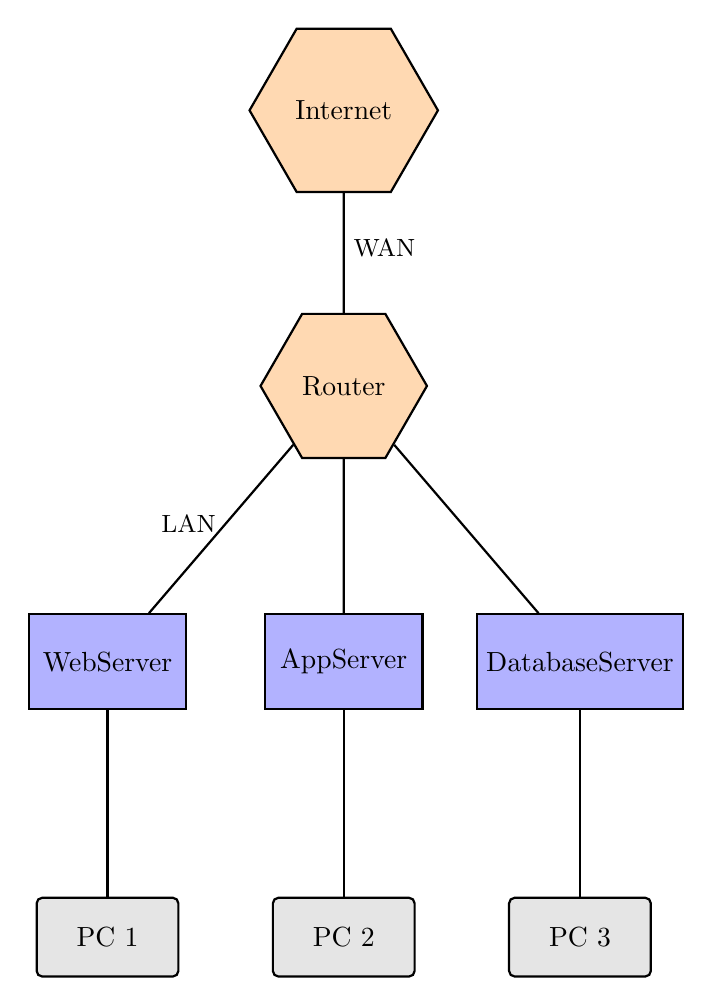
\begin{tikzpicture}[
    node distance=2.5cm,
    server/.style={rectangle, minimum width=2cm, minimum height=1.2cm,
                   text centered, draw=black, thick, fill=blue!30},
    router/.style={regular polygon, regular polygon sides=6, minimum size=1.5cm,
                   draw=black, thick, fill=orange!30},
    computer/.style={rectangle, rounded corners=2pt, minimum width=1.8cm, minimum height=1cm,
                     text centered, draw=black, thick, fill=gray!20},
    line/.style={thick}
]

    % Internet and router
    \node (internet) [router] {Internet};
    \node (router) [router, below of=internet, yshift=-1cm] {Router};

    % Servers
    \node (web) [server, below of=router, xshift=-3cm, yshift=-1cm] {Web\\Server};
    \node (app) [server, below of=router, yshift=-1cm] {App\\Server};
    \node (db) [server, below of=router, xshift=3cm, yshift=-1cm] {Database\\Server};

    % Client computers
    \node (pc1) [computer, below of=web, yshift=-1cm] {PC 1};
    \node (pc2) [computer, below of=app, yshift=-1cm] {PC 2};
    \node (pc3) [computer, below of=db, yshift=-1cm] {PC 3};

    % Connections
    \draw [line] (internet) -- (router);
    \draw [line] (router) -- (web);
    \draw [line] (router) -- (app);
    \draw [line] (router) -- (db);
    \draw [line] (web) -- (pc1);
    \draw [line] (app) -- (pc2);
    \draw [line] (db) -- (pc3);

    % Labels on connections
    \node[right, font=\small] at ($(internet)!0.5!(router)$) {WAN};
    \node[left, font=\small] at ($(router)!0.5!(web)$) {LAN};

\end{tikzpicture}
\end{center}

\section{State Machine Diagram}

\begin{center}
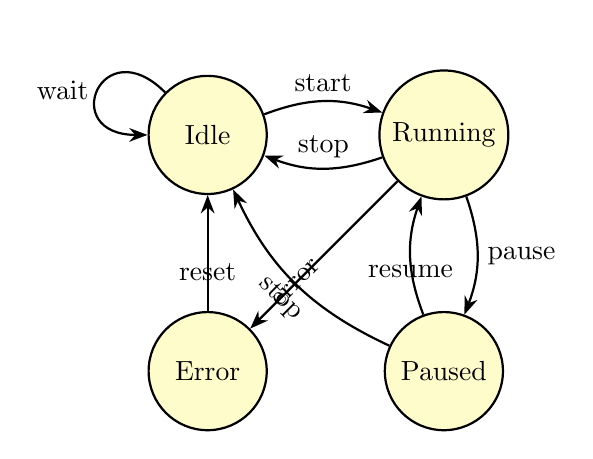
\begin{tikzpicture}[
    node distance=3cm,
    state/.style={circle, minimum size=1.5cm, thick, draw=black, fill=yellow!20},
    arrow/.style={->,>=Stealth,thick,bend angle=20}
]

    % States
    \node (idle) [state] {Idle};
    \node (running) [state, right of=idle] {Running};
    \node (paused) [state, below of=running] {Paused};
    \node (error) [state, below of=idle] {Error};

    % Transitions
    \draw [arrow, bend left] (idle) to node[above] {start} (running);
    \draw [arrow, bend left] (running) to node[right] {pause} (paused);
    \draw [arrow, bend left] (paused) to node[below] {resume} (running);
    \draw [arrow, bend left] (running) to node[above, sloped] {stop} (idle);
    \draw [arrow, bend left] (paused) to node[below, sloped] {stop} (idle);
    \draw [arrow] (running) to node[left, sloped] {error} (error);
    \draw [arrow] (error) to node[below] {reset} (idle);

    % Self-loop
    \draw [arrow] (idle) to [out=135,in=180,looseness=5] node[left] {wait} (idle);

\end{tikzpicture}
\end{center}

\section{Class Diagram}

\begin{center}
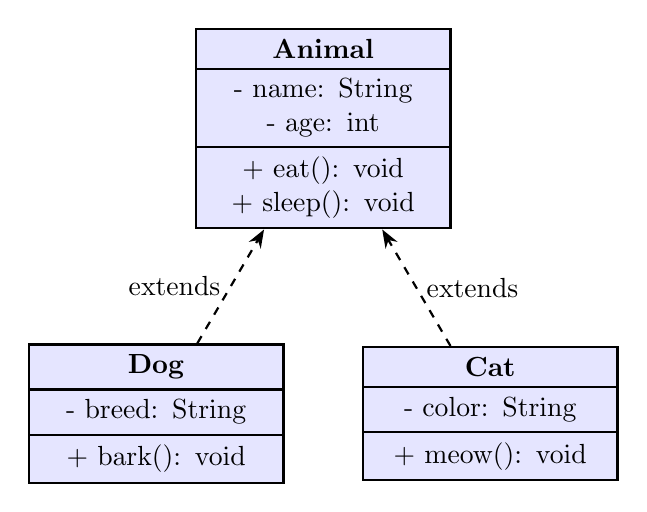
\begin{tikzpicture}[
    node distance=3cm,
    class/.style={rectangle split, rectangle split parts=3,
                  draw=black, thick, text width=3cm, align=center,
                  fill=blue!10},
    arrow/.style={->,>=Stealth,thick}
]

    % Classes
    \node (animal) [class] {
        \textbf{Animal}
        \nodepart{second}
        - name: String\\
        - age: int
        \nodepart{third}
        + eat(): void\\
        + sleep(): void
    };

    \node (dog) [class, below left of=animal, yshift=-1.5cm] {
        \textbf{Dog}
        \nodepart{second}
        - breed: String
        \nodepart{third}
        + bark(): void
    };

    \node (cat) [class, below right of=animal, yshift=-1.5cm] {
        \textbf{Cat}
        \nodepart{second}
        - color: String
        \nodepart{third}
        + meow(): void
    };

    % Inheritance arrows
    \draw [arrow, dashed] (dog) -- (animal) node[midway, left] {extends};
    \draw [arrow, dashed] (cat) -- (animal) node[midway, right] {extends};

\end{tikzpicture}
\end{center}

\section{Mind Map}

\begin{center}
\begin{tikzpicture}[
    mindmap,
    grow cyclic,
    every node/.style={concept, execute at begin node=\hskip0pt},
    root concept/.style={concept color=blue!30, font=\Large\bfseries, minimum size=2.5cm},
    level 1 concept/.style={concept color=green!30, sibling angle=90, minimum size=2cm, font=\normalsize},
    level 2 concept/.style={concept color=orange!30, minimum size=1.5cm, font=\small}
]

    \node [root concept] {Machine\\Learning}
        child [concept color=red!30] { node {Supervised\\Learning}
            child { node {Classification} }
            child { node {Regression} }
        }
        child [concept color=blue!30] { node {Unsupervised\\Learning}
            child { node {Clustering} }
            child { node {Dimensionality\\Reduction} }
        }
        child [concept color=green!30] { node {Deep\\Learning}
            child { node {CNN} }
            child { node {RNN} }
        }
        child [concept color=yellow!50] { node {Reinforcement\\Learning}
            child { node {Q-Learning} }
            child { node {Policy\\Gradient} }
        };

\end{tikzpicture}
\end{center}

\section{Compilation Notes}

To compile this document:
\begin{verbatim}
pdflatex tikz_diagram.tex
\end{verbatim}

Complex diagrams may require longer compilation times.

\end{document}
